\begin{center}
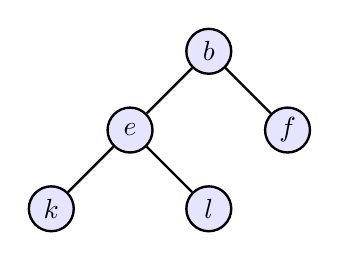
\begin{tikzpicture}

\fill[blue!10] (9.0, -1.0) circle (0.3);
\node [line width=0.03cm,black,minimum size=0.57cm,draw,circle] at (9.0,-1.0)(b){};\draw (9.0, -1.0) node[color=black] {$b$};
\fill[blue!10] (8.0, -2.0) circle (0.3);
\node [line width=0.03cm,black,minimum size=0.57cm,draw,circle] at (8.0,-2.0)(e){};\draw (8.0, -2.0) node[color=black] {$e$};
\fill[blue!10] (10.0, -2.0) circle (0.3);
\node [line width=0.03cm,black,minimum size=0.57cm,draw,circle] at (10.0,-2.0)(f){};\draw (10.0, -2.0) node[color=black] {$f$};
\fill[blue!10] (7.0, -3.0) circle (0.3);
\node [line width=0.03cm,black,minimum size=0.57cm,draw,circle] at (7.0,-3.0)(k){};\draw (7.0, -3.0) node[color=black] {$k$};
\fill[blue!10] (9.0, -3.0) circle (0.3);
\node [line width=0.03cm,black,minimum size=0.57cm,draw,circle] at (9.0,-3.0)(l){};\draw (9.0, -3.0) node[color=black] {$l$};\draw[line width=0.03cm,black] (b) to  (e);
\draw[line width=0.03cm,black] (b) to  (f);
\draw[line width=0.03cm,black] (e) to  (k);
\draw[line width=0.03cm,black] (e) to  (l);
\end{tikzpicture}

\end{center}

